%!TEX root = PhD_Thesis.tex
\chapter[Segmentation from 3D Ultrasound]{Segmentation of Steerable Needles from 3D Ultrasound Image Data}

%%%%%%%%%%%%%%%%%%%%%%%%%%%%%%%%%%%%%%%%%%%%%%%%%%%%%%%%%%%%%%%%%%%%%%%%%%%%%%%%%%%%%%%%%%%%%%%%%%%%======================================================================
\section{Introduction}
%======================================================================
%%%%%%%%%%%%%%%%%%%%%%%%%%%%%%%%%%%%%%%%%%%%%%%%%%%%%%%%%%%%%%%%%%%%%%%%%%%%%%%%%%%%%%%%%%%%%%%%%%%
This chapter describes methods for automatic segmentation of steerable needles from 3D ultrasound data. The work presented in this chapter was previously published in the IEEE Transactions on Biomedical Engineering~\cite{Adebar2014}.

CT imaging, magnetic resonance (MR) imaging and X-ray imaging could all potentially be applied to intraoperative guidance of steerable needles, but each of these modalities has significant drawbacks. Our work uses 3D ultrasound because of its many advantages. Ultrasound systems image in real time, do not produce ionizing radiation, and are not strongly affected by the presence of metal objects such as needles. Perhaps most importantly, ultrasound systems are inexpensive and portable, and are already standard equipment in existing operating rooms and treatment suites.  

Ultrasound does have disadvantages, such as low signal-to-noise ratio and poor image resolution compared to MR or CT. When imaging needles, ultrasound image quality is highly dependent on the angle between the ultrasound imaging plane and the needle. At some angles, significant reverberation artifacts generated by the highly reflective needle surfaces may appear. At other angles, the needle may not be visible at all, as the reflected waves may be dispersed away from the transducer~\cite{Chung2004}. Even when the needle can be identified, various imaging artifacts can make it difficult to locate the tip of the needle along its axis. 

The underlying issue that makes automatic needle segmentation a difficult problem is the poor visibility of needles in standard B-mode ultrasound data. Several methods for B-mode segmentation have shown promising results in favorable conditions. However, image-guided robotic needle steering requires segmentation algorithms that can process large 3D datasets containing highly curved, extremely thin (e.g., 0.6-mm diameter) needles at undesirable orientations relative to the transducer. Rather than contribute a new algorithm that attempts to overcome these challenges, our aim in this chapter was to reduce the complexity of the segmentation task, by leveraging the needle steering robot to produce ultrasound image data that more clearly reveal the needle.

Ultrasound Doppler is a diagnostic technique that measures frequency shifts in reflected ultrasonic waves that result from motion. Color and power Doppler imaging, which are available on most modern ultrasound systems, are commonly applied to overlay blood flow data on B-mode ultrasound, as described in Section~\ref{sec:Doppler-BasedSegmentation}. Vibrating solid objects have also been shown to produce recognizable Doppler signals~\cite{Holen1985}. This concept has been applied to localize straight needles~\cite{Armstrong2001,Feld1997,Hamper1991} and needle tips~\cite{Harmat2006} in 2D ultrasound, as well as instruments in cardiac interventions~\cite{Fronheiser2008,Reddy2008} and other applications~\cite{McAleavey2003,Rogers2009}. This technique has not previously been applied to segment highly curved needles.

\begin{figure}[!t]
\centering
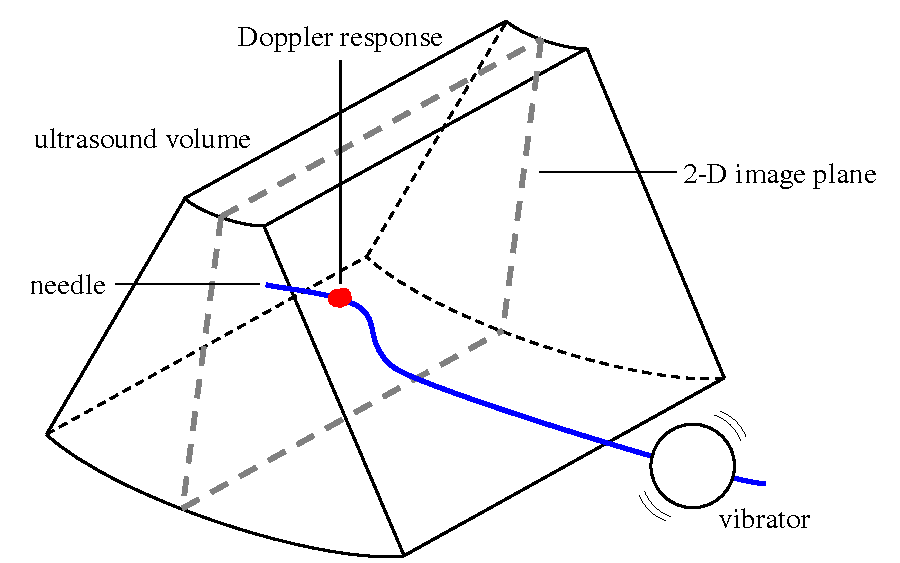
\includegraphics[width = 0.75\columnwidth]{Images/Chapter2/SliceConcept/SliceConcept}%
\caption[3D ultrasound segmentation concept]{Needle segmentation concept. A voice coil actuator (vibrator) vibrates the needle, resulting in a Doppler response around the needle cross section in a 2D ultrasound image. The needle is segmented by localizing the Doppler response across the sweep of a mechanical 3D ultrasound transducer, and fitting a curve through the resulting points.}
\label{fig:SliceConcept}
\end{figure}

The remainder of this chapter is divided into four sections. Section~\ref{sec:Algorithms} describes our Doppler segmentation approach. Section~\ref{sec:Closed-loopControlDoppler} describes a closed-loop control approach, which incorporates the segmentation results as feedback. Variations of this control approach will also be applied in later chapters. Section~\ref{sec:ExperimentalValidation} describes experimental methods for validation of our segmentation and control algorithms. Section~\ref{sec:Results} presents and discusses the results of the validation testing.

\section{Segmentation Algorithm}
\label{sec:Algorithms}
Throughout the description of our segmentation algorithm, we will assume that the needle is oriented roughly orthogonal to the imaging plane of a mechanical 3D ultrasound transducer, as depicted in Fig.~\ref{fig:SliceConcept}. An actuator is used to vibrate the needle, and the resulting motion of the needle and surrounding tissue produces a Doppler signal across the series of $N$ Doppler images generated by the ultrasound system. Segmentation proceeds in two stages, as depicted in Fig.~\ref{fig:Segmentation}. First, the cross section of the needle is localized in each image through 2D image processing. Second, the 3D shape of the needle is reconstructed by fitting a curve to the series of points.

\subsection{2D Image Processing}
To remove Doppler noise, patches with less than 300 connected pixels are removed. (For comparison, the Doppler patch centered around the needle typically has a connected area of 1000 to 2000 pixels.) After this preprocessing step, the image coordinates of the needle cross section are estimated based on the remaining Doppler response. As seen in the example image in Fig.~\ref{fig:Segmentation}, the Doppler response from the vibration generally appears as an irregular, roughly circular patch centered on the needle, with a color comet tail artifact in the axial ($y_\text{image}$) direction~\cite{Tchelepi2009}. The lateral ($x_\text{image}$) coordinate of the needle is thus estimated as the centroid of the Doppler response. To account for the color comet tail, the axial image coordinate of the needle is estimated as the point that separates one quarter of the integral of the Doppler response above, and three quarters below. These fractions were selected empirically based on the results of our feasibility study~\cite{Adebar2013}. 

We define the $x$, $y$, and $z$ directions of the 3D ultrasound coordinate system to be in the lateral, axial, and elevational directions, respectively. Based on the geometry of the ultrasound transducer, the needle points are mapped from the 2D image coordinate system to the 3D ultrasound coordinate system, yielding the set of $N$ needle points $d^{(0)}, \dotsc, d^{(N)}$. Each $d^{(i)} \in \mathbb{R}^{3}$ holds the $x$-$y$-$z$ coordinates of detected needle point~$i$.

\begin{figure*}[!t]
\centering
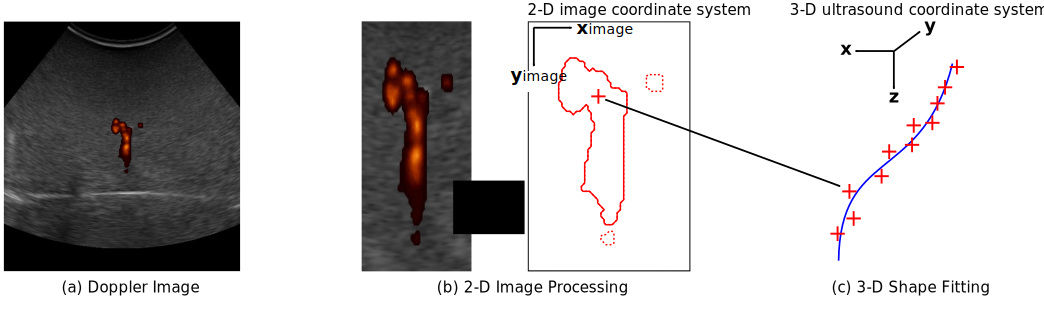
\includegraphics[width = \textwidth]{Images/Chapter2/Segmentation/Segmentation}%
\caption[Doppler ultrasound segmentation algorithm]{Segmentation algorithm: (a) Doppler image. A 2D ultrasound Doppler image from a series of $N$ captured over a sweep of the imaging plane. (b)~2D image processing. Doppler patches with fewer than 300 connected pixels are assumed to be noise and discarded (dotted lines). The remaining Doppler data (solid line) are used to estimate the position of the needle cross section (cross). In the lateral ($x_\text{image}$) direction, the position is estimated as the centroid of the Doppler response. In the axial ($y_\text{image}$) direction, the position is estimated as the lower bound of the region that contains one quarter of the integrated Doppler intensity. (c) 3D shape fitting. The 2D-localized points are combined in 3D based on position information from the 3D ultrasound transducer. Third-order polynomial curves are fit to the identified points in order to define the needle's 3D shape over the series of $N$ images.}
\label{fig:Segmentation}
\end{figure*}

\subsection{3D Shape Fitting}
Based on the Doppler points identified in the previous step, we resolve the shape of the needle by defining the $x$ and $y$ coordinates as functions of the $z$ coordinate over the range of $d^{(0)}, \dotsc, d^{(N)}$. In this work we use third-order polynomial functions,
\begin{align}
d^{(i)}_x = f_x(d_z^{(i)}) = a_0 + a_1(d_z^{(i)}) + a_2(d_z^{(i)})^{2} + a_3(d_z^{(i)})^{3},\notag\\
d^{(i)}_y = f_y(d_z^{(i)}) = b_0 + b_1(d_z^{(i)}) + b_2(d_z^{(i)})^{2} + b_3(d_z^{(i)})^{3},\label{result}
\end{align}
and solve for the vectors of polynomial coefficients $a,b \in \mathbb{R}^{4}$ that minimize the sum of the squared error over the measured Doppler points. We selected this curve type because a third-order polynomial was sufficient to represent the range of curved needle paths we considered in this study. Additionally, low-order polynomials have the advantage that they average out noise in the 2D Doppler points, which is important in our method. Longer, more tortuous paths might require more sophisticated curves, possibly segmented polynomials constrained to be tangent at transition points.

\begin{figure}[!t]
\centering
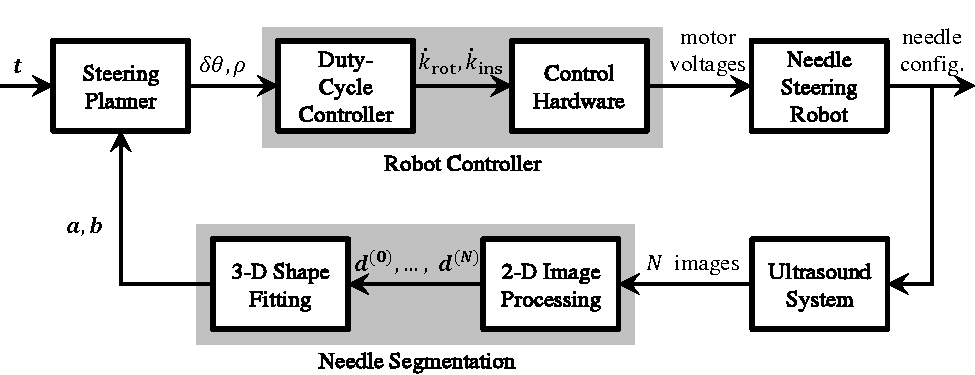
\includegraphics[width=\columnwidth]{Images/Chapter2/ControlBlockDiagram/ControlBlockDiagram}%
\caption[Block diagram of closed-loop control algorithm]{Block diagram of closed-loop control in ultrasound-guided needle steering. Automatic segmentation of the needle from 3D ultrasound data provides a measurement of needle tip pose to a steering controller, which identifies the needle rotation and curvature necessary to reach a target point. A duty-cycle controller generates the velocity commands that allow motor control hardware to move the needle tip along the desired path to the target.}
\label{fig:ControlBlockDiagram}
\end{figure}

\section{Closed-loop Control Algorithm}
\label{sec:Closed-loopControlDoppler}
To demonstrate the usefulness of the Doppler ultrasound segmentation method described in the previous section, we implemented closed-loop control of a needle steering robot using the ultrasound segmentation results as feedback. Fig.~\ref{fig:ControlBlockDiagram} shows a block diagram. The goal of the closed-loop control is to steer the needle tip towards a target point ${t}$ defined in the ultrasound coordinate system. The same general framework for closed-loop control will be used in Chapters 4 and 5, with some modifications. Implementation of closed-loop control necessitated two new algorithmic components in addition to needle segmentation: tip pose measurement and a steering controller. 

The pose of the needle tip, defined by position $p$ and orientation $R$, is measured by interpreting the needle segmentation results. In this chapter, the tip pose measurement is based on a small-angle approximation. This approximation is appropriate for the range of needle steering paths described in this chapter, which are representative of ablation shaping around a single tumor. In Chapter 4, we describe an estimation scheme based on an unscented Kalman filter, which allows position feedback to be combined with a kinematic model of needle tip motion, in order to estimate the complete tip pose. This estimation scheme enables longer paths steering through a large workspace in the liver. 

The steering controller interprets the tip pose measurement, and determines a desired path for the steerable needle that will cause it to reach the target. In this chapter, a simple replanning approach, previously described by Majewicz and Okamura~\cite{Majewicz2013}, was employed. This approach has the limitation that it requires duty-cycle control of needle curvature; however, it is sufficient to demonstrate accurate closed-loop steering for the small paths described in this chapter. In Chapter 5, we apply the sliding mode control described in~\cite{Rucker2013}, which does not rely on duty-cycle control.

The tip frame measurement algorithm and steering controller, as well as the robotic system used to validate them, are described in detail in the remainder of this section. 

\subsection{Tip Pose Measurement}
We define the needle tip frame as shown in Fig.~\ref{fig:ControlAlgorithm}. The origin of the tip frame is located at point ${p}$, which is the distal end of the needle. For simplicity, we ignore the local geometry of the bent tip. The tip frame has orientation represented by rotation matrix $R$, with the $z_{\text{tip}}$ axis tangent to the needle at ${p}$, and the $y_{\text{tip}}$ axis pointing in the direction of curvature. The center of curvature for the circular needle path ${c}$ lies on the $y_{\text{tip}}$-axis, at a distance $\rho$ from ${p}$. Using duty-cycle control~\cite{Minhas2007}, $\rho$ can be varied from $\rho_{\text{min}}$ to $\infty$ (a straight line).  

%In our model, rotating the base of the needle by $\delta\theta$ causes the needle tip frame to rotate by $\delta\theta$ about the $z_{\text{tip}}$ axis, while inserting the needle causes the tip point ${p}$ to move along  a circular path of radius $\rho$.

Based on the segmentation result, the tip point ${p}$ is identified using the $z$ coordinate of the most distal Doppler point and the polynomial curve functions,
\begin{align}
{p} = \begin{bmatrix}p_x & p_y & p_z\end{bmatrix}^{\text{T}} = \begin{bmatrix}f_x(d^{(0)}_z) & f_y(d^{(0)}_z) & d^{(0)}_z \end{bmatrix}^{\text{T}}.
\end{align}
While it should also be possible to estimate the tip frame orientation $R$ based on the needle segmentation result, for example by fitting a circular arc to a curved section of the 3D segmentation result to define the steering direction, we have found that in the current implementation the Doppler segmentation results are too noisy to allow reliable estimation of the tip frame orientation. Instead we apply a small angle approximation, and assume that the $z_{\text{tip}}$ axis remains close to the $z$ axis of the 3D ultrasound coordinate system throughout steering. The orientation of the tip frame can thus be specified completely by a rotation of $\theta$ about the $z$ axis. We make rotation angle $\theta$ a system variable, and update it after each iteration of the steering controller, 
\begin{align}
\theta_\text{i+1} = \theta_\text{i} + \delta\theta_\text{i}.
\end{align}
This approach ignores torsional deflection of the steerable needle as result of friction between the needle and tissue. While substantial torsional deflection has been demonstrated in artificial tissues, in biological tissues the needle tip rotation has been shown to follow the base rotation to within a few degrees~\cite{Reed2008}. 

\subsection{Steering Controller}
At each iteration, the steering controller interprets the tip pose measurement, defined by $p$ and $R$, and identifies the simplest possible path to the target point ${t}$. As shown in Fig.~\ref{fig:ControlAlgorithm}, this path is the circular arc that is tangent to the measured $z_{\text{tip}}$ axis at $p$, and passes through ${t}$. The radius of the desired path $\rho_{\text{des}}$ and the incremental needle rotation $\delta\theta$ needed to follow the path are output to the robot controller, which drives the motors of the needle steering robot.

\begin{figure}[!t]
\centering
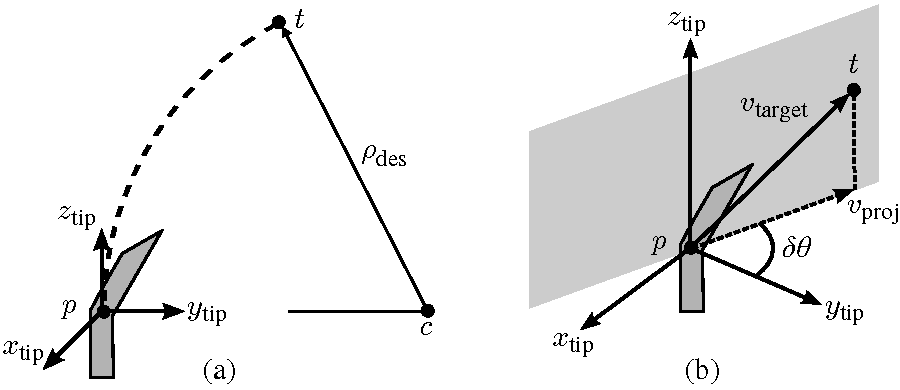
\includegraphics[width = 0.75\columnwidth]{Images/Chapter2/ControlAlgorithm/ControlAlgorithm}%
\caption[Steering controller]{Steering controller: (a) The needle tip frame is located at the distal end of the needle. The frame is oriented with the $z_{\text{tip}}$ axis tangent to the needle, and the $y_{\text{tip}}$ axis pointing towards the center of curvature. The needle follows a circular path, with radius $\rho$ which can be varied using duty-cycle control. (b) The steering controller determines the incremental rotation $\delta\theta$ and the desired path radius $\rho_{\text{des}}$ that will cause the needle tip $p$ to reach the target point ${t}$.}
\label{fig:ControlAlgorithm}
\end{figure}

\subsection{Robot Controller} 
The robot controller consists of two components. A duty-cycle controller generates motor velocity commands based on the desired needle rotation and radius of curvature as output by the steering controller. Motor control hardware drives the motors of the needle steering robot based on the velocity commands.

\subsubsection{Duty-Cycle Controller}
The goal of the duty-cycle controller is to determine the desired velocities for the rotation and insertion stages, $\dot{k}_\text{rot}$ and $\dot{k}_\text{ins}$. It is first necessary to calculate the duty-cycle fraction $DC$, based on the desired radius of curvature. Assuming a known minimum radius of curvature $\rho_\text{min}$ for the specific needle-tissue pair, $DC$ can be calculated as,
\begin{align}
DC = 1.0 - \frac{\rho_\text{min}}{\rho_{\text{des}}}. 
\label{eq:DC}
\end{align}
The insertion velocity, $\dot{k}_\text{ins}$, is set to a constant value during steering.  To achieve the duty-cycle effect, the rotation stage alternates between constant velocity, $\dot{k}_\text{rot} = \dot{k}_\text{rot, max}$, and zero velocity, $\dot{k}_\text{rot} = 0$, with the needle held at angle $\theta$. The ratio of time spent rotating ($T_\text{rot}$) to time holding at angle $\theta$ ($T_\text{hold}$) is determined from the duty cycle ratio $DC$,
\begin{align}
DC =\frac{T_\text{rot}}{T_\text{rot}+T_\text{hold}}.
\end{align}
Rotation time $T_\text{rot}$ is constant and equal to the time required to complete a full rotation. Hold time $T_\text{hold}$ is thus varied to achieve the desired ratio $DC$.

\subsubsection{Control Hardware}
There are many possible hardware implementations that could be used to drive the motors of the needle steering robot. In the system we use for experimental validation in Section~\ref{sec:ExperimentalValidation}, the rotation and insertion motors are each driven by integrated motion control systems. These systems accept velocity commands (i.e., $\dot{k}_\text{rot}, \dot{k}_\text{ins}$) and drive the motors using proportional-integral (PI) control. In our system, PI control constants were tuned using manufacturer supplied software.

\section{Experimental Validation}
\label{sec:ExperimentalValidation}
In this section, we describe experimental validation of our algorithms for segmentation and closed-loop 3D ultrasound-guided needle steering.
\subsection{Apparatus}
%Figure~\ref{fig:Setup} shows our experimental apparatus.
\subsubsection{Ultrasound Imaging}
A SonixMDP ultrasound console (Ultrasonix Medical Corp., Richmond, Canada) with a convex mechanical 3D transducer (4DC7-3/40) was used for imaging. Custom software incorporating the Ultrasonix research SDK package was used to control imaging parameters and capture images. Power Doppler imaging mode was selected over color Doppler imaging because of the lack of aliasing and reduced sensitivity to imaging angle. Pulse repetition frequency (PRF) was set to 1428 Hz, as this setting yielded the best results in our initial feasibility study~\cite{Adebar2013}. Wall motion filter (WF) was set to maximum in order to minimize Doppler artifacts resulting from the motion of the imaging plane. Each sweep consisted of 61 scan-converted 2D images, captured at angular increments of approximately 0.7 degrees.

\begin{figure*}[!t]
\centering{
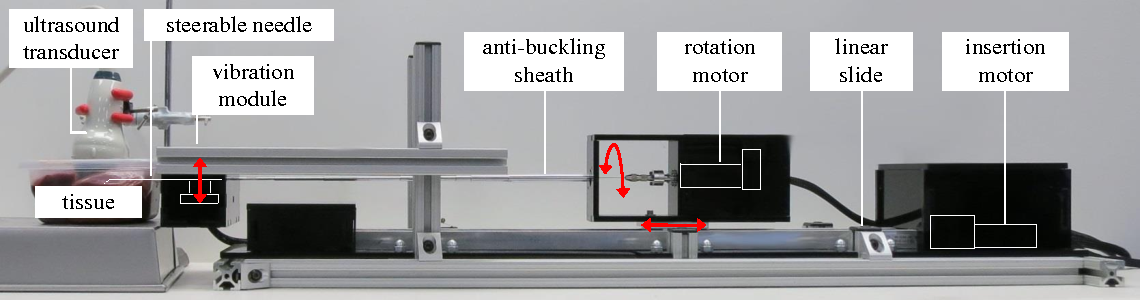
\includegraphics[width=\textwidth]{Images/Chapter2/RobotSetup/RobotSetup}%
}
\caption[Experimental setup]{Experimental setup. Needle steering robot consisting of actuated linear slide, rotation stage, and vibration module (red arrows indicate actuation); \textit{ex vivo} bovine liver tissue; 3D ultrasound transducer.}
\label{fig:ExperimentalSetup}
\end{figure*}

\begin{figure}[!t]
\centering{
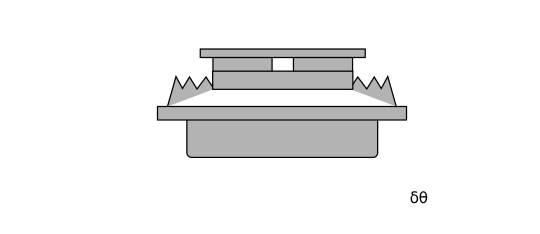
\includegraphics[width = 0.7\columnwidth]{Images/Chapter2/Vibrator/Vibrator}%
}
\caption[Vibration module]{Vibration module. A voice coil actuator is attached to the steerable needle using a 3D-printed clip, and used to vibrate the needle vertically (in and out of the page).}
\label{fig:Vibrator}
\end{figure}

\subsubsection{Needle Steering Robot}
Fig.~\ref{fig:ExperimentalSetup} shows the needle steering robot used to validate our control method. Similar to previously described needle steering robots~\cite{Webster2005}, our system has two active degrees of freedom (DOF) that control needle insertion and needle rotation. Unlike previous needle steering robots, our system incorporates a vibration module that generates the high-frequency motion necessary to visualize the needle using ultrasound Doppler.

The rotational DOF is actuated by a geared DC motor (A-max 22-110160; Maxon Motor, Sachseln, Switzerland) that is connected directly to the needle through a pin-vise clamp. The insertion DOF is actuated by a DC motor (GM9234S016; Ametek, Berwyn, PA) that drives a linear slide (SPMA2524W4; VelMex, Bloomfield, NY). Both the rotation DOF and insertion DOF are driven by integrated motion controllers (MCDC3006S; Faulhaber, Schönaich, Germany). The vibration module, shown in Fig.~\ref{fig:Vibrator}, consists of a voice coil actuator (HIAX19C01-8; HiWave, Little Gransden, UK) that is driven by a transistor circuit at a user-variable frequency of 400~Hz, 600~Hz or 800~Hz. These frequencies are roughly centered around the peak output point of the voice coil actuator and thus produce the strongest responses in the power Doppler image data. To produce the maximum vibration along the needle, the vibration module was designed to be as close as possible to the target tissue, and is thus attached to the distal end of the needle steering robot. The needle is mated to the actuator using a 3D-printed plastic clip.

\subsubsection{Needles}
Solid Nitinol wires 0.38~mm (0.015~inches), 0.48~mm (0.019~inches) and 0.58~mm (0.023~inches) in diameter were used as needles. The needles had 45-degree beveled tips and 4.5-mm distal sections bent 35 degrees off axis.

\subsubsection{Tissue Simulant}
\textit{Ex vivo} bovine liver tissue obtained fresh from a local butcher was used as the tissue simulant in all testing.

\subsection{Segmentation Accuracy}
We previously described a feasibility study~\cite{Adebar2013}, in which we measured the accuracy of our Doppler segmentation method using piezoelectric elements welded to stainless-steel wires. In that study, we examined the sensitivity of the method to tissue composition, vibration frequency, and Doppler PRF, and found that only PRF greatly affected the accuracy of segmentation. Based on comparison with manual segmentation, we found the average error to be 1 to 2~mm across most conditions.

In this study, we evaluated the accuracy of segmentation when using an actual needle steering robot with an integrated actuator to vibrate flexible Nitinol needles. We again considered the impact of vibration frequency, although at a lower range than our previous experiment because of the lower center frequency of the voice coil actuator compared to the previous piezoelectric actuator. We also considered the impact of needle curvature, needle diameter, and position of the needle in the lateral image direction. Two needle curvatures (straight and maximum curvature), two lateral positions (image center and lateral edge), three needle diameters (0.38~mm, 0.48~mm, and 0.58~mm), and three vibration frequencies (400~Hz, 600~Hz, and 800~Hz) were tested. Each parameter was varied individually around the base case of a straight, 0.48-mm needle centered in the image and vibrated at 600~Hz. 

Three separate insertions and scans were performed for each test condition. Segmentation accuracy was evaluated by comparison with a reference manual segmentation of the needle from B-mode data, within the native image planes of the 3D ultrasound transducer. To create the reference data, the center of the needle was manually selected in each 2D B-mode image in which it was visible. The needle was visible in approximately 50 percent of the B-mode images captured over most sweeps. 

Given $K$ manually selected needle points ${m}^{(0)}, \dotsc, {m}^{(K)}$, we defined the segmentation error for the $i$-th point,
\begin{equation}
e^{(i)} = \sqrt{ \left(m_x^{(i)}-f_x(m_z^{(i)})\right)^2 + \left(m_y^{(i)}-f_y(m_z^{(i)})\right)^2.} 
\end{equation}
\noindent For this segmentation accuracy testing, the Doppler segmentation method and the reference manual segmentation were both implemented in Matlab.

The precision of the reference data was quantified by measuring variability between repeated manual segmentations of the same B-mode volumes. Although this does not measure the absolute accuracy of the reference data, it provides an indication of manual segmentation error. Across four repeated segmentations each for eight needle scans (four of straight needles and four of curved needles), the standard distance deviation, 
\begin{equation}
S_{xy} = \sqrt{      \sum_{i=1}^{M} \frac{(d^{(i)}_{\text{MC}})^2}{M-2}       },
\end{equation}
\noindent was calculated, where $d^{(i)}_{\text{MC}}$ is the distance in the image plane between the $i$-th manually selected needle point and the corresponding mean center, and $M$ is the total number of comparison points. With $M =$~684 data points, we found the standard distance deviation for the manual segmentation to be $S_{xy} =$~0.23~mm.

\subsection{Closed-Loop Steering}
We validated the needle segmentation algorithm and steering controller in a series of needle steering tests. The algorithms described above were implemented in C++ using the ITK and VTK libraries~\cite{ITK2002} for image analysis. Six insertion tests were performed, using 0.48-mm needles with bent tips as described above. In each test, a brachytherapy sheath was used to insert a cylindrical stainless steel bead into a liver tissue specimen, in order to generate a target. The beads were 3 mm in diameter and 5 mm long, and were oriented for maximum visibility in the 3D B-mode images (i.e., with the long axis of the beads approximately perpendicular to the axial direction of the ultrasound) to enable the manual reference segmentation. The 3D ultrasound transducer was applied to the tissue and oriented so that the target was near the boundary of the ultrasound volume in the $z$ (elevational) direction. The steerable needle was then inserted until it was just visible at the opposite end of the ultrasound volume. The initial position of the steerable needle tip, ${p}$, relative to the target, ${t}$, was varied within a rectangular workspace with approximate dimensions of 20~mm by 20~mm by 30~mm. This workspace is representative of ablation shaping for medium-sized liver tumors (between 30~mm and 50~mm in diameter) using a single RF electrode, assuming a rigid needle or other introducer was used to initially place the steerable needle near the target. The dimensions of the needle steering path for each closed-loop steering test are listed in Section~\ref{sec:Results}. The initial orientation of the steerable needle tip was such that the tip frame was aligned with the ultrasound coordinate system (i.e., $\theta = 0$ degrees). After these initial insertion steps, a 3D ultrasound volume was captured, and the bead was manually segmented to yield the position of the target in the 3D ultrasound frame. Point ${t}$ was placed on the surface of the bead closest to the starting position of the needle tip. The needle was then automatically steered towards the target until the system detected that the needle tip had reached the target depth in the $z$ direction, at which point insertion was stopped. Targeting error was measured as the 3D distance between the target point ${t}$ and the needle tip ${p}$ at the end of the test.

In this study, the control algorithm depicted in Fig.~\ref{fig:ControlBlockDiagram} was implemented in discrete increments. The control inputs of rotation and duty cycle were held constant over increments of insertion. At the end of each increment, insertion was stopped, and the needle was vibrated, scanned, and segmented automatically. The steering controller was then applied to determine the rotation and duty cycle inputs for the following increment. Relatively large 5-mm insertion increments were selected for testing to reduce deformation of the tissue due to needle stiction. Insertion velocity, $\dot{k}_\text{ins}$, was set to yield a linear needle insertion rate of 100 mm/min. Maximum rotation velocity, $\dot{k}_\text{rot, max}$, was set to yield a rotary needle velocity of 60~RPM.

Minimum radius of curvature $\rho_{\text{min}}$ for the 0.48-mm needle in \textit{ex vivo} bovine liver tissue was measured in a separate initial experiment. The steerable needle was inserted into the liver without rotation, scanned and segmented, and a circular arc was fit to the segmentation results. Over four repetitions, the average radius of curvature was found to be 51.4~mm, which is within the range of curvature values previously reported in \textit{ex vivo} tissue~\cite{Majewicz2012}. This was the value of $\rho_{\text{min}}$ used by the duty cycle controller to calculate the duty cycle ratio $DC$ based on the desired radius of curvature.
 
\section{Results and Discussion}
\begin{figure*}[!t]
\centering
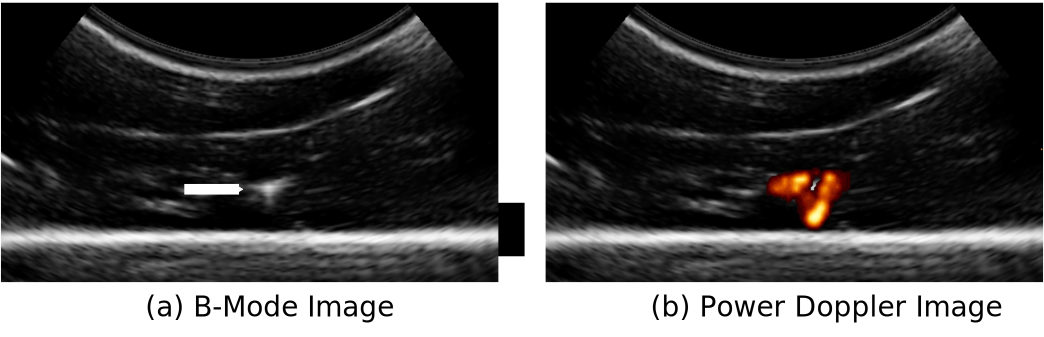
\includegraphics[width=\textwidth]{Images/Chapter2/2DUS/2DUS}%
\caption[2D ultrasound images from 3D sweeps of needle]{2D ultrasound images taken from volumetric sweeps of steerable needles inserted into \textit{ex vivo} liver: (a) B-mode ultrasound image used for manual segmentation. The needle cross section is indicated. (b) Corresponding power Doppler ultrasound image captured during needle vibration. The Doppler response surrounds the needle cross section.}
\label{fig:2DUS}
\end{figure*} 

\label{sec:Results}
Fig.~\ref{fig:2DUS} shows example 2D ultrasound images taken from volumetric sweeps of steerable needles in \textit{ex vivo} liver. Both B-mode and power Doppler images are shown. The needle cross section was visible in approximately 50 percent of the B-mode images captured over most sweeps. As shown in the figure, the high-frequency vibration of the needle causes a power Doppler response centered around the needle cross section.

\begin{figure*}[!t]
\centering
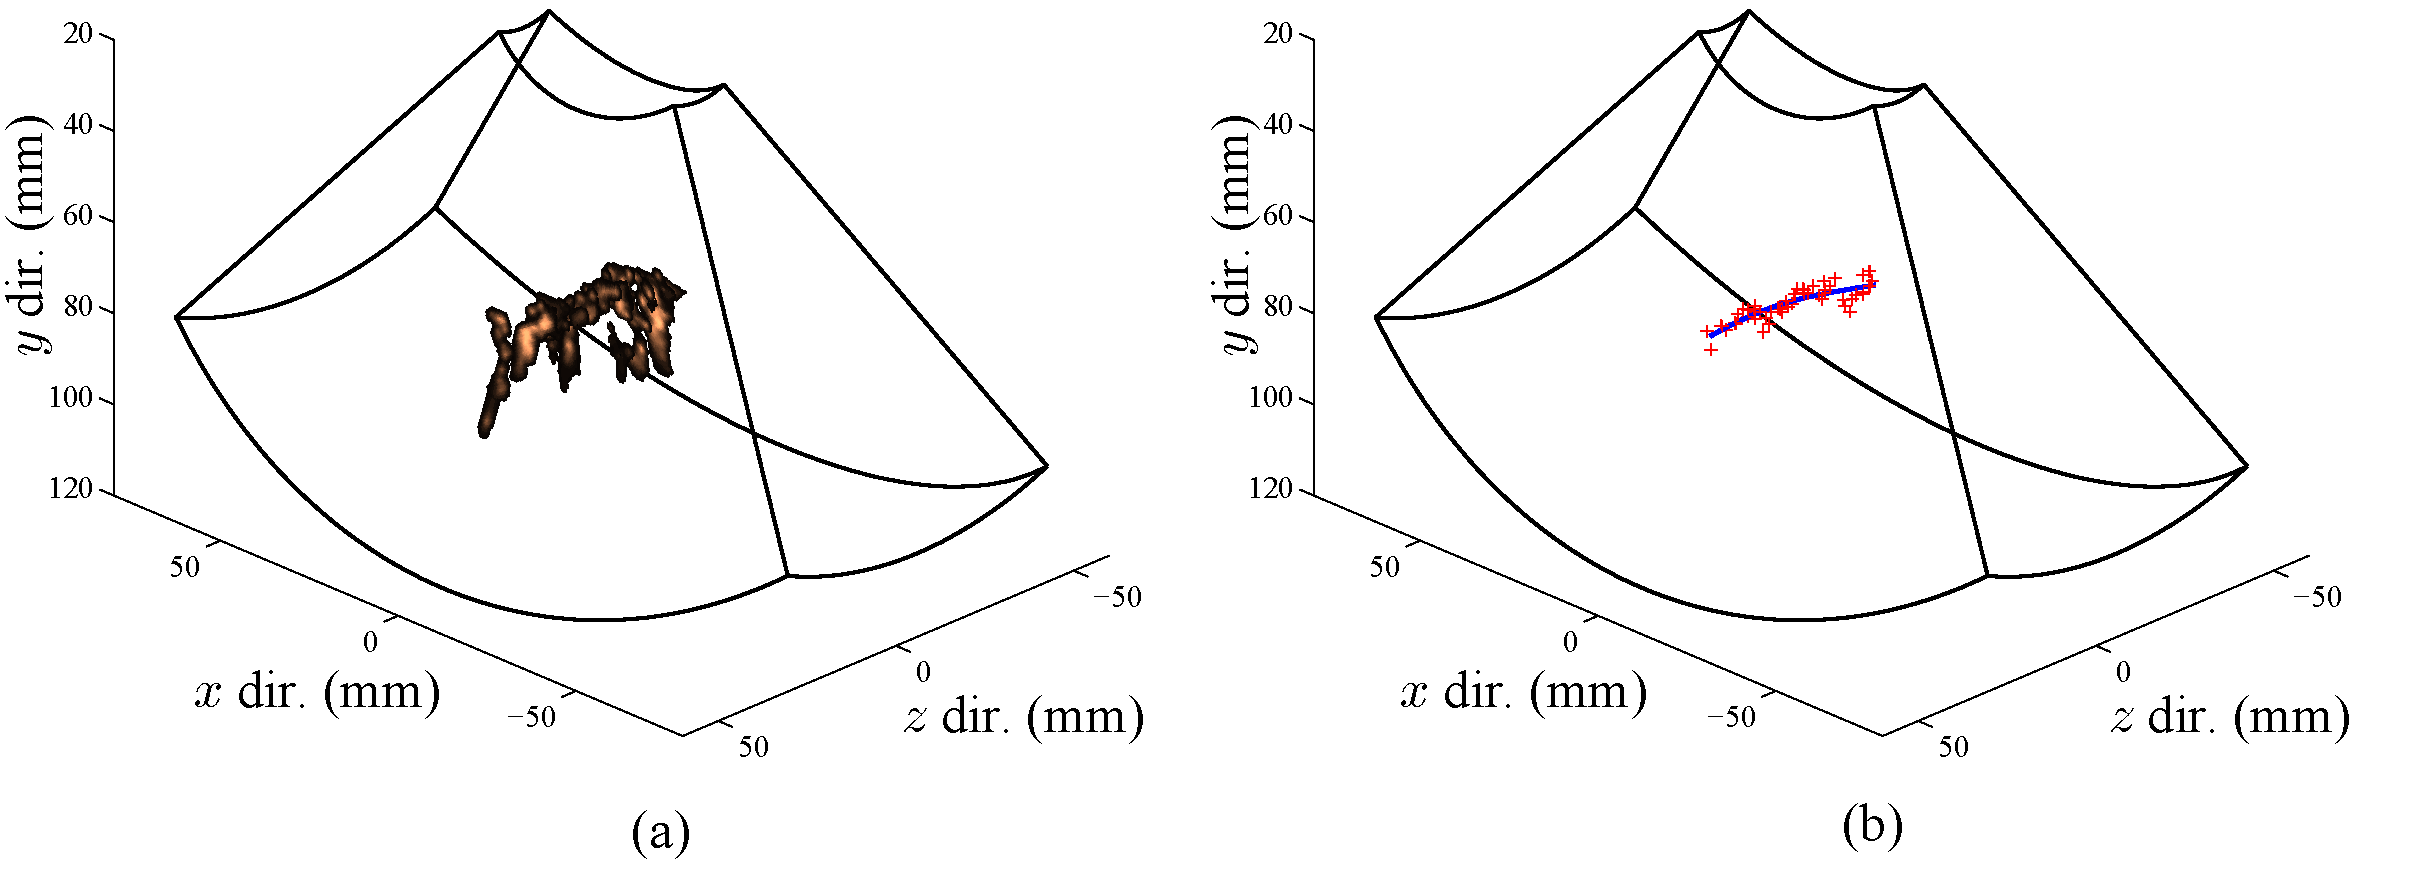
\includegraphics[width=\textwidth]{Images/Chapter2/DopplerVisualization/Doppler3D}%
\caption[Example segmentation of needle using Doppler method]{Example segmentation of needle using Doppler method: (a) Power Doppler response around the needle in each image. (b) Reconstructed needle shape (blue curve), fit through the centroids of the Doppler data in each image (red crosses).}
\label{fig:SegmentationExample}
\end{figure*}   

Fig.~\ref{fig:SegmentationExample} shows the 3D Doppler data generated by a vibrating needle, along with the corresponding Doppler centroids and best-fit polynomial curve. Volumetric framerate using the SonixMDP system was 0.2~Hz for power Doppler data at an imaging depth of 50~mm. Software runtimes were approximately 60~ms per image for the 2D image processing algorithm and 15~ms per sweep for the steering controller, when implemented on the SonixMDP's integrated processor.

\subsection{Segmentation Accuracy}
Fig.~\ref{fig:SegmentationError} summarizes the results of the segmentation accuracy tests. Across all tests, the maximum segmentation error was 3.18~mm, the minimum segmentation error was 0.13~mm, the mean segmentation error was 1.24~mm, and the standard deviation of the segmentation error was 0.57~mm. In the base case tests (straight, 0.48-mm needle centered in the image and vibrated at 600~Hz), the mean segmentation error was 0.92~mm and the standard deviation of the segmentation error was 0.93~mm.

In the needle curvature test, curved and straight needles had similar segmentation errors, with somewhat higher errors in the curved configuration. The mean error was 0.85~mm for straight needles, and 1.36~mm for curved needles. We conclude that for transducers initially oriented as shown in Fig.~\ref{fig:SliceConcept}, our segmentation method is suitable for the range of needle geometries that can be achieved by bent tip steering in biological tissue (assuming $\rho_{\text{min}} \approx$ 50~mm). The implementation described in this chapter fails if the steerable needle is exactly parallel to the imaging plane, thus presenting a linear rather than circular cross section. However, this can be avoided by placing the 3D transducer so the needle is initially approximately perpendicular to the imaging plane. Applying the Doppler segmentation technique without constraint on the transducer orientation, and with other 3D ultrasound implementations---such as freehand tracked 3D ultrasound---is addressed in Chapter 4.

\begin{figure*}[!t]
\centering
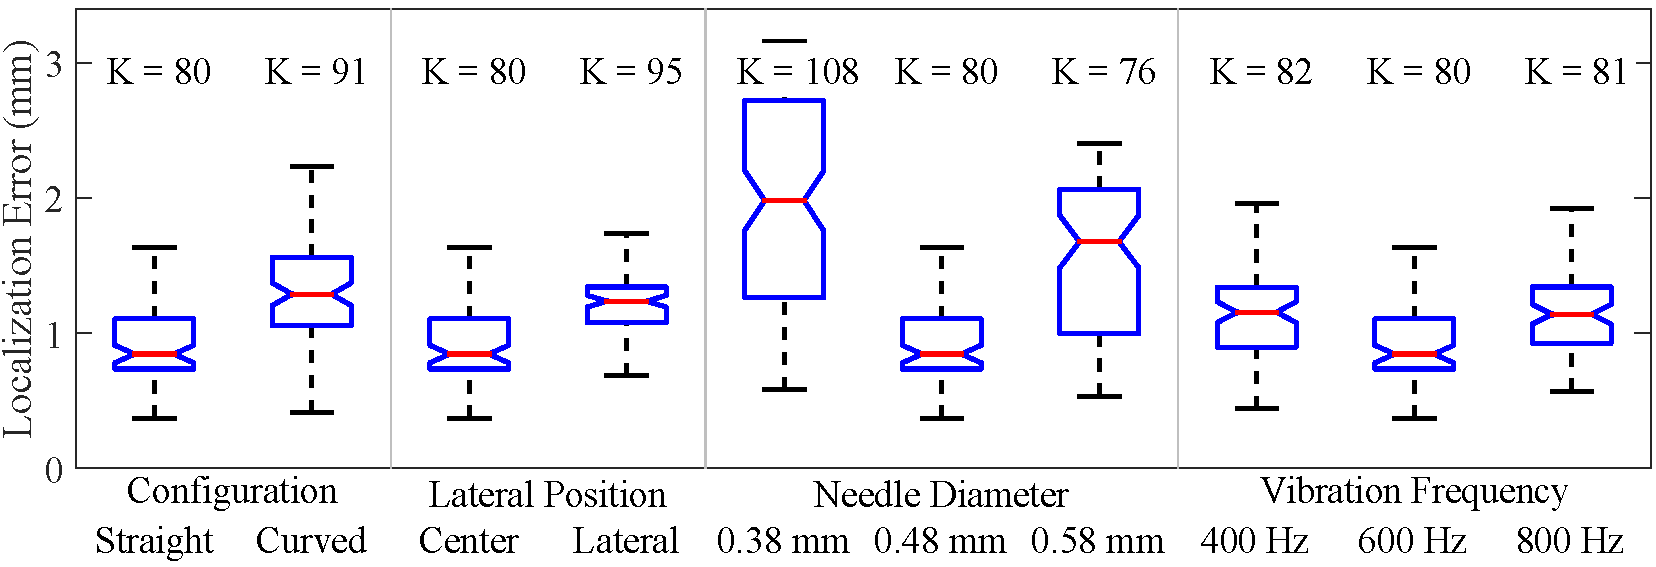
\includegraphics[width=\textwidth]{Images/Chapter2/SegmentationAccuracy/SegmentationAccuracy}%
\caption[Doppler segmentation accuracy results]{Segmentation accuracy results. Two needle configurations (straight, curved), two image positions (center, lateral), three needle diameters (0.38~mm, 0.48~mm, 0.58~mm), and three vibration frequencies (400~Hz, 600~Hz, 800~Hz) were tested. For each group, red line indicates median error, blue box indicates 25th and 75th percentile, and whiskers indicate minimum and maximum error. Number of data points for each group is also indicated.}
\label{fig:SegmentationError}
\end{figure*}

Needle diameter had a significant effect on segmentation accuracy. Mean error was 0.85~mm for 0.48-mm needles, versus 1.98~mm for 0.38-mm needles and 1.68~mm for 0.58-mm needles. The significant change in mean error for the 0.48-mm needles is surprising given the relatively small change in needle diameter. The complexity of the wave mechanics that govern the transmission of vibrations along a flexible needle in viscous tissue makes it difficult to theorize why needle diameter appears to be an important factor. This issue is worthy of future study for two reasons. First, because improved understanding of the motion around the vibrating needle might allow for new Doppler processing algorithms that specifically target the generated motion. Second, because specific needle geometries may be required for other clinical applications (for example, brachytherapy systems would likely require hollow needles).

Lateral image position and vibration frequency did not have significant impacts on segmentation accuracy. In the lateral position test, the mean error was 0.85~mm for needles centered in the image, and 1.24~mm for needles on the lateral edge. In the vibration frequency test, the mean error was 1.16~mm for 400-Hz vibration, 0.85~mm for 600-Hz vibration, and 1.14~mm for 800-Hz vibration. In the case of vibration frequency, the insensitivity is in agreement with our previous study~\cite{Adebar2013}, where varying vibration frequency over a much larger range did not significantly affect segmentation accuracy. 

\subsection{Closed-Loop Steering}
Table~\ref{table:Targeting Results} lists results from six successful closed-loop needle steering tests. For each test, the number of insertion increments ($N_{\text{inc}}$), the $x$-$y$-$z$ dimensions of the complete needle steering path ($\delta x$, $\delta y$, and $\delta z$), and the final error in tip placement relative to the target ($e_{\text{final}}$) are listed. Mean tip placement error was 1.57~mm over the six tests, which is close to the mean error in Fig.~\ref{fig:SegmentationError} for that configuration. 

\begin{figure*}[!t]
\centering
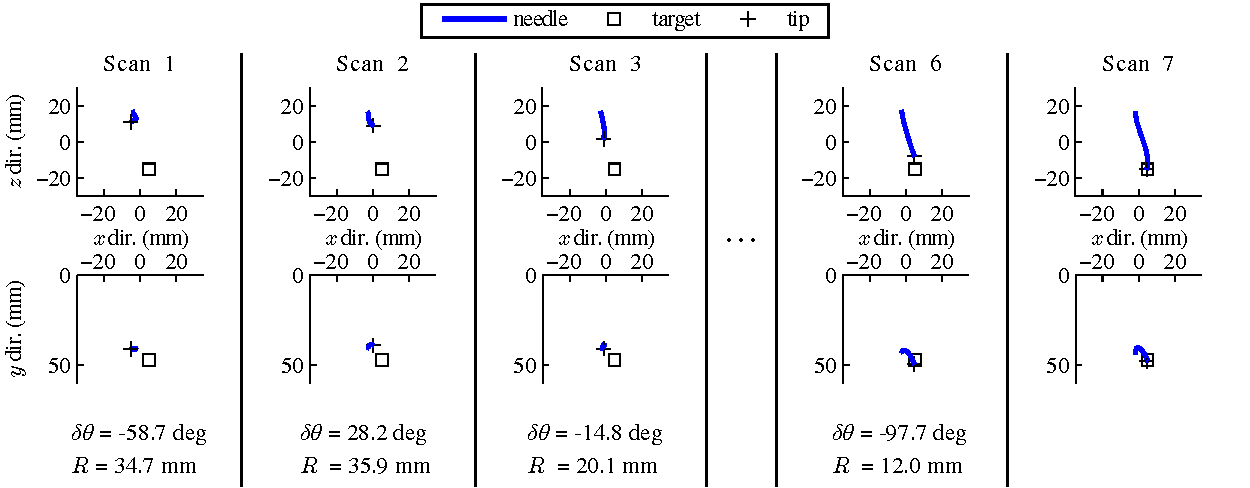
\includegraphics[width = \textwidth]{Images/Chapter2/Steering/Steering}%
\caption[Closed-loop needle steering results]{Closed-loop needle steering results. Orthogonal views of successive incremental scans during needle steering in \textit{ex vivo} tissue, with the output from the steering controller after each scan below. The needle base was inserted 5~mm between each scan, with rotation and duty cycle determined by the steering controller. Error in placing the tip at the target bead was 0.86~mm after the final insertion.}
\label{fig:SucessfulSteering}
\end{figure*}

Fig.~\ref{fig:SucessfulSteering} shows the needle shapes reconstructed during incremental closed-loop steering in Test~6. The $y_{\text{tip}}$-axis was initially aligned with the $y$-axis of the ultrasound coordinate system. After Scan 1, the steering controller compensated by rotating the $y_{\text{tip}}$-axis towards the target ($\delta\theta = -58.7 \text{ degrees}$). The steering controller gave smaller corrections based on Scans 2 to 5, as a result of deviation from the steering model and noise in the measurement of point ${p}$. After Scan 6, when the needle tip was within several millimeters of the target, the steering controller output a large unnecessary rotation correction ($\delta\theta = -97.7 \text{ degrees}$), but over such a small distance it had little effect. Final tip placement error $e_{\text{final}}$ was 0.86~mm for this test.

\begin{table}[!t]
% increase table row spacing, adjust to taste
\renewcommand{\arraystretch}{1.3}
\centering
\caption{Closed-loop needle steering results}
\label{table:DopplerTargetingResults}
% Some packages, such as MDW tools, offer better commands for making tables
% than the plain LaTeX2e tabular which is used here.
\begin{tabulary}{\columnwidth}{| c | C | C | C | C | C |}
\hline
Test & $N_{\text{inc}}$ \newline  & $\delta x$ \newline (mm) & $\delta y$ \newline (mm) & $\delta z$ \newline (mm) & $e_{\text{final}}$\newline (mm)\\
\hline
1 	& 6 &	1.99   &   10.74  &   29.09  &	1.57    \\
\hline
2 	& 7 &	8.42   &   7.15   &   29.16  &	1.73	\\
\hline
3 	& 6 &	7.81   &   2.63   &   31.44  &	1.27	\\
\hline
4 	& 6 &	8.04   &   6.81   &   31.78  &	2.08    \\
\hline
5	& 6 &	1.75   &   5.06   &   26.46  & 	1.89    \\
\hline
6 	& 6 &	6.13   &   3.83   &   32.26  &	0.86    \\
\hline
\end{tabulary}
\end{table}

In addition to the six tests listed in Table~\ref{table:DopplerTargetingResults}, there were several tests which failed as a result of poor needle steering behavior. Bent-tip needle steering requires a homogeneous solid medium. If the steerable needle tip impacts an obstacle which it does not pierce through, such as a bone or blood vessel, the path of the needle may deviate greatly from what is expected. Fig.~\ref{fig:Steering} shows the reconstructed needle shapes from one such failed test. In this test, the needle appeared to impact one of several small vessels that could be visualized in ultrasound before the final scan. Fig.~\ref{fig:LiverVessel} shows examples of these small vessels in a section of liver specimen.

\begin{figure*}[!t]
\centerline{\subfigure[ ]{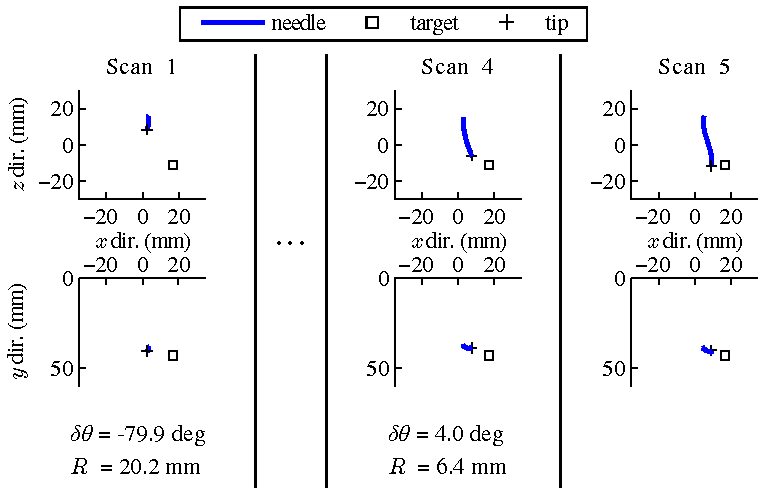
\includegraphics[width = 0.6\textwidth]{Images/Chapter2/FailedSteering/Steering}%
\label{fig:Steering}}
\hfil
\subfigure[ ]{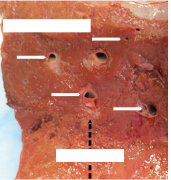
\includegraphics[height=2.2in]{Images/Chapter2/FailedSteering/LiverVessel}%
\label{fig:LiverVessel}}}
\caption[Closed-loop needle steering results; failed steering trial]{Closed-loop needle steering results. Example of failed needle steering: (a) Orthogonal views of successive incremental scans during needle steering in \textit{ex vivo} tissue, with the output from the steering controller after each scan below. The needle base was inserted 5~mm between each scan, with rotational orientation and duty cycle setting determined by the steering controller outputs. Error in placing the tip at the target bead was 8.14~mm after the final insertion. The needle failed to reach the target due to interference from internal vessels that could  be visualized in the ultrasound images. (b) Section of tissue sample with example vessels and approximate direction of needle insertion indicated.}
\label{fig:FailedSteering}
\end{figure*}

\subsection{Discussion}
The methods described in this chapter are capable of segmenting a curved needle with average error of 1 to 2~mm, and steering a needle to a target with an average error of 1.57~mm. This is roughly equivalent to manual targeting error with medical image guidance, which has been shown to be 2~mm or higher on average~\cite{Crocetti2008,MaierHein2008,Schubert2013}. Studies of percutaneous RFA of liver cancer generally suggest that an ablative margin of 5-10~mm around a tumor is necessary to prevent recurrence of cancer~\cite{Dodd2001,Kim2006,Gervais2009}. However recent work has reported that ablative margins as small as 3~mm are associated with a lower rate of local tumor progression~\cite{Kim2010}. This suggests that a targeting error of 2~mm may be tolerable. Overall, the experimental results described in this chapter show that our segmentation and control algorithms approach the accuracy and consistency necessary for a practical clinical application such as RFA of liver cancer. 

In this chapter, we applied our segmentation and control algorithms to sequences of incremental insertions, rather than to constant velocity insertions. We believe this is the most realistic approach in a clinical setting. Although a delay of several seconds for ultrasound scanning after each incremental insertion might seem undesirable to roboticists, it actually mirrors current clinical practice where clinicians frequently pause during needle insertion to take CT scans. 

Needle vibration in this chapter is achieved by an actuator connected to the proximal end of the steerable needle. In this implementation, the Doppler response decreases moving along the needle towards the tip, as the vibrations are damped out by the surrounding tissue. For very long insertion paths, or more viscous tissues, the amplitude of vibration at the tip might be too small to allow a reliable Doppler segmentation. We are currently exploring other actuation schemes that vibrate the needle tip directly, as in~\cite{Harmat2006} or~\cite{McAleavey2003}, although integrating these actuators into sub-millimeter steerable needles is a difficult practical problem.

With vibration of the needle, the added potential for tissue damage is an issue that must be considered carefully. Unfortunately, both the tissue strain around the vibrating shaft and the displacement of the sharp needle tip are difficult to measure experimentally, and it was not possible to quantify these factors in the current work. Histological analysis after steering in an \textit{in vivo} model, as in~\cite{Majewicz2012}, would likely be required to evaluate tissue damage. As stated above, the displacement of the needle shaft is in the sub-millimeter range at the needle base, and decreases along the needle shaft due to tissue damping. While we thus expect the resulting tissue damage to be minimal, this issue is again worthy of further study.

It should be noted that the duty cycling approach we apply to control steerable needle curvature has largely been validated in homogeneous artificial tissues, although several examples of duty cycling in biological tissues have been reported~\cite{Swaney2013,Engh2010,Patil2014}. Recent work~\cite{Patil2014} suggests that the linear relationship between duty cycle and curvature described in Equation (\ref{eq:DC}) may oversimplify steerable needle behavior in heterogeneous biological tissue. Fortunately the closed-loop structure of our steering algorithm compensates for deviation from the expected relationship, and for variation in $\rho_\text{min}$.